%The building is treated as a lumped-parameter system, which assumes nodes in the room as well as in the walls, floor, and ceiling describing the respective temperatures.
%Considering the heat transfer rate between the nodes, an equivalent thermal RC network is identified. 
%The influence of the actuators is modeled according to their heat transfer properties, e.g. the heating input from the radiator goes directly into the room node, whereas floor heating affects the room with some delay and therefore the control input from floor heating goes into the node in the floor.

The bilinear model has 12 internal states including the inside zone temperature $\mathsf{T}_{\mathrm{in}}$, the slab temperatures $\mathsf{T}_{\mathrm{sb}}$, the inner wall $\mathsf{T}_{\mathrm{iw}}$ and the outside wall temperature $\mathsf{T}_{\mathrm{ow}}$. The state vector is defined as $x:=[\mathsf{T}_{\mathrm{in}}, \mathsf{T}_{\mathrm{sb}}^{(1:5)}, \mathsf{T}_{\mathrm{ef}}^{(1:3)}, \mathsf{T}_{\mathrm{in}}^{(1:3)}]^T$.

There are 4 control inputs including the blind position $\mathsf{B}$, the gains due to electric lighting $\mathsf{L}$, the evaporative cooling usage factor $\mathsf{C}$, and the heat from the radiator $\mathsf{H}$ such that $u:=[\mathsf{B},\mathsf{L},\mathsf{H},\mathsf{C}]^T$. $\mathsf{B}$ and $\mathsf{L}$ affect both room illuminance and temperature due to heat transfer whereas $\mathsf{C}$ and $\mathsf{H}$ affect only temperature.

The model is subject to 5 weather disturbances: solar gains with fully closed blinds $\mathsf{Q}_{\mathrm{sc}}$ and with open blinds $\mathsf{Q}_{\mathrm{so}}$, daylight illuminance with open blinds $\mathsf{I}_{\mathrm{o}}$, external dry-bulb temperature $\mathsf{T}_{\mathrm{db}}$ and external wet-bulb temperature $\mathsf{T}_{\mathrm{wb}}$. 
The hourly weather forecast, provided by MeteoSwiss, was updated every 12 hrs. Therefore, to improve the forecast,  an autoregressive model of the uncertainty was considered.
Other disturbances come from the internal gains due to occupancy $\mathsf{Q}_{\mathrm{io}}$ and due to equipments $\mathsf{Q}_{\mathrm{ie}}$ which were assumed as per the Swiss standards \cite{Merkblatt2006}. We define $d:=[\mathsf{Q}_{\mathrm{sc}},\mathsf{Q}_{\mathrm{so}},\mathsf{I}_{\mathrm{o}},\mathsf{Q}_{\mathrm{io}},\mathsf{Q}_{\mathrm{ie}},\mathsf{T}_{\mathrm{db}},\mathsf{T}_{\mathrm{wb}}]^T$. For further details, we refer the reader to \cite{Oldewurtel2011}.

The model dynamics are given below. The bilinearity is present in both input-state, and input-disturbance.
\begin{gather}
\label{E:bilinear1}
x_{k+1} = Ax_{k}+(B_u +B_{xu}[x_k] + B_{du}[d_k]) u_k+B_dd_k \\
x_{k} \in \mathbb{R}^{12}, u_{k} \in \mathbb{R}^{4}, d_{k} \in \mathbb{R}^{8} \ \forall k = 0,\dots,T, \nonumber
\end{gather}
where, the matrices $B_{xu}$ and $B_{du}$ are defined as
\begin{gather}
\label{E:bilinear2}
B_{xu}[x_k] = [ B_{xu,1}[x_k],B_{xu,2}[x_k], \dots, B_{xu,4}[x_k] ] \in \mathbb{R}^{12\times4}, \nonumber\\
B_{du}[d_k] = [ B_{du,1}[d_k],B_{du,2}[d_k], \dots, B_{du,4}[d_k] ] \in \mathbb{R}^{12\times4}\nonumber, \\
B_{xu,i} \in \R^{12\times12}, B_{du,i} \in \R^{12\times8} \ \forall i=1,2,3,4.\nonumber
\end{gather}
For this study, we assume that the disturbances are precisely known to MPC as well as DPC controller. In our future work, we will account for the uncertainties in the disturbances with an extension to Scenario approach \cite{Bernardini2009} for DPC.

\begin{figure}[t!]
	\centering
	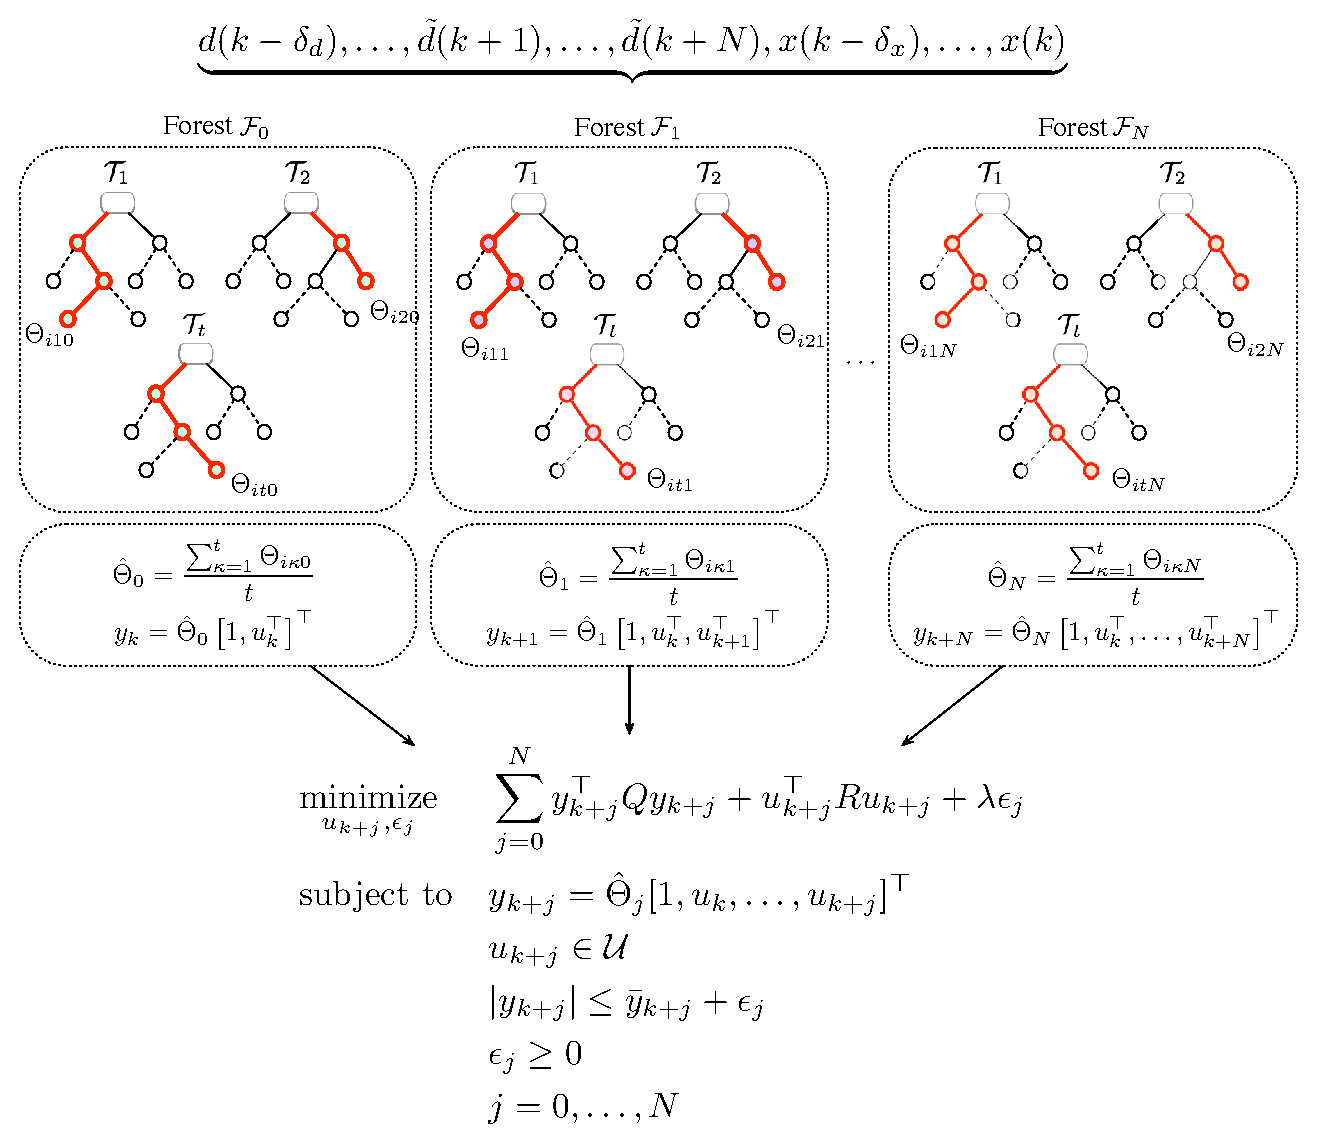
\includegraphics[width=21pc]{figures/dpc-algo-rf.eps}
	\caption{DPC-En: At time $k$, the algorithm uses the forecast of disturbances $\tX^d_{\mathrm{k|k}}$ to select linear models $\Theta_1$ to $\Theta_t$ in the leaves of each ensemble. The linear models in each ensemble are averaged to calculate a single model represented by $\hat{\Theta}_j$ which act as constraints in the optimization problem. The optimal sequence $[\tX^c_{\mathrm{k|k}},\dots,\tX^c_{\mathrm{k+N-1|k}}]$, of which the first one is applied, and $\tX^d_{\mathrm{k+1|k+1}}$ is calculated to proceed to $k+1$.}
	\label{F:dpc-algo-rf}
\end{figure}